\documentclass[11pt, oneside]{article}   	% use "amsart" instead of "article" for AMSLaTeX format
\usepackage{geometry}                		% See geometry.pdf to learn the layout options. There are lots.
\usepackage[parfill]{parskip}    			% Activate to begin paragraphs with an empty line rather than an indent
\usepackage{graphicx}						% Use pdf, png, jpg, or eps§ with pdflatex; use eps in DVI mode
											% TeX will automatically convert eps --> pdf in pdflatex
\usepackage{amssymb}
\usepackage{hyperref} 						% for \hyperfootnote
\usepackage{pifont}							% for \ding
\usepackage{url}							% for "plainurl" support in \bibliographystyle 

% Make clickable footnote
\newcommand{\hyperfootnote}[1][]{\def\ArgI{{#1}}\hyperfootnoteRelay}
	% relay to new command to make extra optional command possible
\newcommand\hyperfootnoteRelay[2][]{\href{#1#2}{\ArgI}\footnote{\href{#1#2}{#2}}}
	% the first optional argument is now in \ArgI, the second is in #1
% Takes at most 3 parameters (see http://www.tex.ac.uk/FAQ-twooptarg.html for info on multiple optional parameters)
% If first parameter isn't given, it's value is '' (empty string in text before footnote reference)
% If second parameter isn't given, it's value is '' (string before visible URL, e.g. 'http://')
% Makes a clickable footnote (alternatively: \url{}) with optional reference in the text as well
% Use 1: \hyperfootnote{www.mywebsite.com}: creates a footnote consisting of a clickable URL
% Use 2: \hyperfootnote[My website]{www.mywebsite.com}: creates a clickable piece of text in the text ('My website') plus a footnote consisting of a clickable URL
% Note: requires the hyperref package.
% Note: use xspace package to add/absorb spaces when necessary (e.g. to avoid a space between the footnote number and a punctuation mark)
% Info on how to define a LaTeX command: https://www.sharelatex.com/learn/Commands

\geometry{letterpaper}                   	% ... or a4paper or a5paper or ... 
\title{Digital Self-Ownership}
\author{Paul Trevithick, The Mee Foundation}
\date{Created March 27, 2023. Revised \today}							
\begin{document}
\maketitle
\begin{abstract}
	Digital self-ownership is a set of individual rights that give people ownership over their online personal information. These rights are related to, but different from property rights involved in the ownership of personal property. We show how these rights be implmented by through a combination of user agents and contract law.
\end{abstract}

\section{Ownership as a system of rights}
Ownership of property is a system of rights. Consider a spoon that you own. Your rights to use the spoon, give it away, sell it, destroy it, and so on, are not intrinsic to the spoon--they exist because they are recognized by law.

John Locke argued that property law should be applied to people. He is commonly regarded as the originator of ``self-ownership''--the idea that humans have a property right in their person. In 1689 he wrote, ``Every man has a property in his own person: this nobody has any right to but himself."\cite{Locke1689}. This idea was taken up by the American revolutionaries, and was instrumental in justifying their passion to be self-sovereign citizens instead of subjects of King George. Locke considered these to be inate human rights.

\section{Digital Self-Ownership}

Today, a few hundred years later, the self-ownership that Locke argued was “self-evident” does not hold in the digital realm. Despite recent advances in privacy law, we still have little control over our digital selves. Much of our human information (e.g., preferences, interests, affiliations, friends, medical records, location data) is collected by corporations involved in surveillance capitalism\cite{zuboff2019}. It is held, bought, sold, and leveraged for the corporation’s economic advantage, not ours. The resulting loss of privacy and lack of a sense of ownership of our personal data is well-known. Although we're not quite ready to go to war over the idea, we believe that owning our digital selves is vitally important to civil society and the survival of democracy in a digital age. 

Digital Self-Ownership (DSO) is an extension of Locke's self-ownership that covers people's digital selves, i.e. their personal information. DSO proposes a set of digital personal rights which establish people's power and control over their personal information. In much the same way that private property gives individuals power over their own belongings, DSO is about increasing the power of individuals relative the power of digital service providers. 

Many argue that the concept of ownership and property should not be applied to data in general\footnote{For other arguments against using the concept of ownership and propertization of personal data (and data in general) see RadicalxChange.org's (\url{https://radicalxchange.org}) Data Freedom Act (\url{https://www.radicalxchange.org/media/papers/data-freedom-act.pdf}), which is “…informed by a model of social, overlapping claims to data. This view of data, which challenges more familiar notions of individual data ownership, is echoed by top researchers in the fields of data privacy, security, and network economics.” See also the Technium Data Manifesto \url{https://kk.org/thetechnium/data-manifesto/} whose first tenet reads, “Data cannot be owned. By anybody.”}, and of course not to personal data specifically. For example, Prewitt\cite{Prewitt2021} argues that “data cannot be owned, but must be governed.”  However, by following the tradition of treating ownership and property as a system of rights, we a set of rights can be designed appropriate for the characteristics of personal data.  

DSO is a system of rights to acheive self-ownership in the digital world. As in real life, the specific bundle of rights is tuned to the nature of the thing being owned. For example in real life the rights for personal property are different from those for real property (land). For DSO we vary the rights by based on whether the data in question is \emph{user-held}\cite{Jurcys2021} or app-held. 

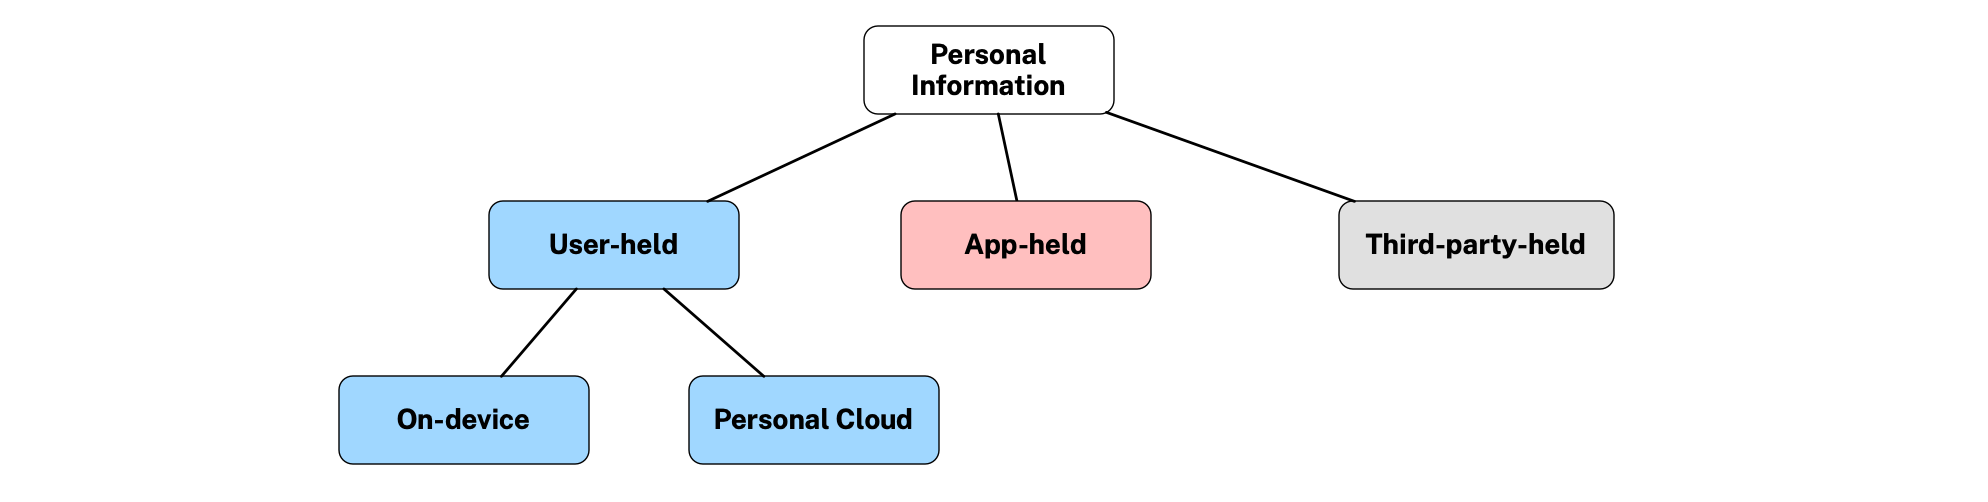
\includegraphics[width=\textwidth]{./images/app-held-user-held-3rd.png}

\emph{Third-party-held} data is data collected and held by third-parties with which the user doens't directly interact and about whom they are often not aware. DSO is not applicable to this kind of data.

\subsection{DSO for User-held Data}

User-held personal information is data about the individual that is created (authored) by them or captured by them using a sensor, and ``held"  (stored) on their personal device such as a phone, personal datastore, or personal data cloud. 

The following is a bundle of rights that taken together provide the user ownership over their user-held data:
\begin{itemize}
	\item \textbf{Assert}. The right to assert information about themself.
	\item \textbf{Access, Update, Delete}. The right to access, update and/or delete their data. 
	\item \textbf{Process}. The right to process their data. This includes leveraging it with local applications, algorithms, and ``personal AI.''  
	\item \textbf{Share}. The right to share data with others without a license. Note that exercising this right undermines ownership, often entirely.
	\item \textbf{License}. The right to transfer a copy of the data to a data custodian's app, whereupon that copy, now being \emph{app-held}, affords the user the rights described below.
\end{itemize}

\subsection{DSO for App-held Data}
App-held data is personal information about an individual that is held (stored) by a digital service provider's mobile app, desktop app, website or webservice with which the individual directly interacts. We call these first-party providers, data custodians.

We define app-held personal information as data that the data custodian has collected through interactions between the individual as a user of the data custodian's app, or through observations made by the app or associated sensors, or through data generated by the app as part of these interactions, but excluding data inferred about the individual as part of these interactions.

In all cases these rights must be implemented through the mechanism of direct digital communication between the data custodian and a user agent. This user agent is the individual's representative in a digital connection with the data custodian.

Below is the minimum bundle of rights that gives the user ownership over their app-held personal data:
\begin{itemize}
	\item \textbf{Opt-in}. The right to require opt-in consent to all collection, transfer, disclosure, retention and use, as well as notification of the data custodian's purpose behind each of these.
	\item \textbf{Access, Update, Delete}. The right, to access update, and delete app-held data held by the data custodian. 
\end{itemize}

\section{Related Work}

Jurcys et al.\cite{Jurcys2021} defined the term \emph{user-held} data and is believed to be the first to describe how self-ownership applies to it. This is closely related to the discussion of user-held data rights above. Van Alstyne et al.\cite{Alstyne2021}'s proposed `In-situ' Data Rights proposal is related to the app-held data rights described above.

The rights we've outlined can be made available to individuals using a combination of legal and technical means. 

\section{Implementation}

\textbf{User-held data rights}

\textbf{Law}. Since user-held data is stored either on a user's own device (phone, tablet, laptop, home server) or in a personal cloud (i.e. a personal datastore in the cloud). In the former case the data is entirely under the user's control. Legal precedent in the United States has supported the notion that a person's phone or other devices is an extension of their physical home and thus its contents protected by the U.S. Constitution from unreasonable searches and seizures by the government. In the later case (user-held data in a peronsal cloud) Jurcys et al.\cite{Jurcys2021} has argued the legal rationale for user ownership.

\textbf{Code}. No special code is required to implement the rights mentioned above. 

\textbf{App-held data rights}

\textbf{Law}. Privacy laws do not recognize the app-held rights we've described\footnote{The situation is in reality even more stark. Putting aside the rights we propose here, individual data ownership rights are not recognized in any jusrisdiction.} we can instead rely on contract law. A contract can be executed between a trusted intermediary operating on behalf of the individual on the one hand, and the first-party data custodian on the other. We call this contract a \emph{Human Information License}. 

\textbf{Code}. A user agent (which by definition represents the user) can consume APIs exposed by the data custodian to implement the access, reading, updating and deleting functions we have described. 

\section{Conclusion}
We have described a system of rights to give individuals ownership over their personal information online. These can be implemented through a combination of contractual and technical means.

\bibliography{../library}
\bibliographystyle{plainurl}
\end{document}  